\section{Analysis}
\textbf{Balance Theory}: 
We investigated the structural compliance of our social network with \textit{structural balance theory} \cite{heider1946attitudes}. 
This theory was recast in a graph-centric manner by Cartwright and Hararay\cite{cartwright1956structural}. 
blah.. blah.. blah..
\subsection{Undirected: Balance Theory}
\begin{figure}
\centering
\subfigure[$T_1$]{
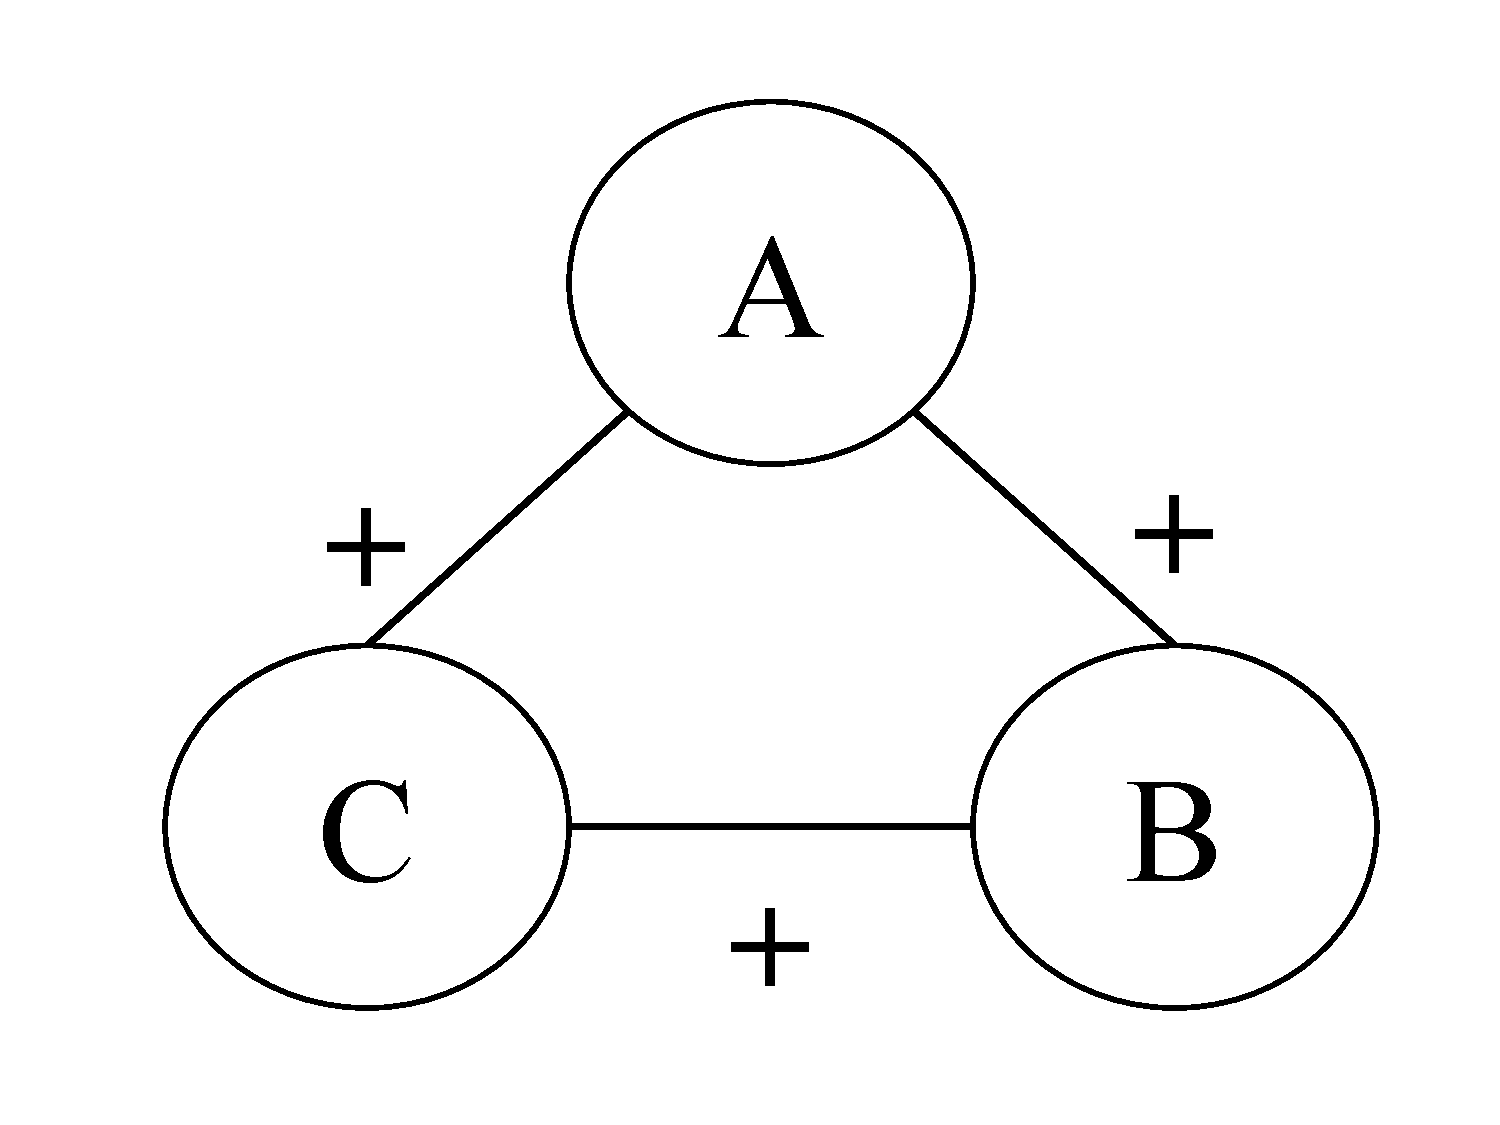
\includegraphics[scale=0.1]{balance_3P0N.pdf}
\label{fig:balance_1P2N}
}
\quad
\subfigure[$T_2$]{
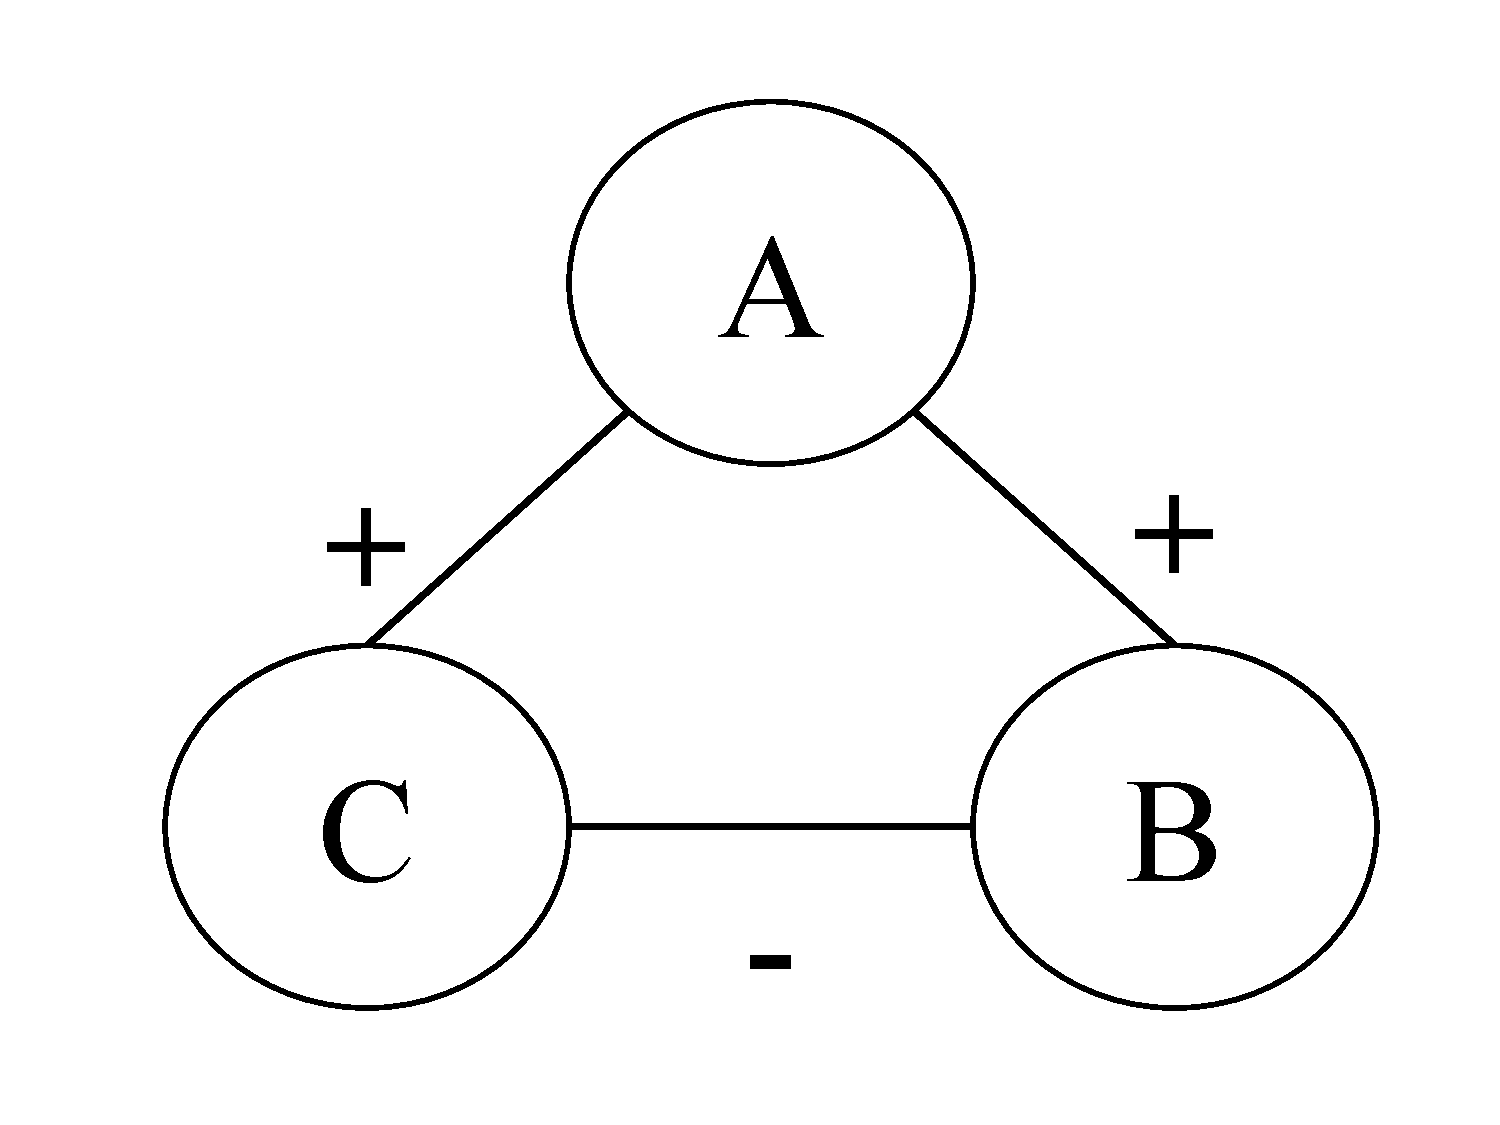
\includegraphics[scale=0.1]{balance_2P1N.pdf}
\label{fig:balance_1P2N}
}

\subfigure[$T_3$]{
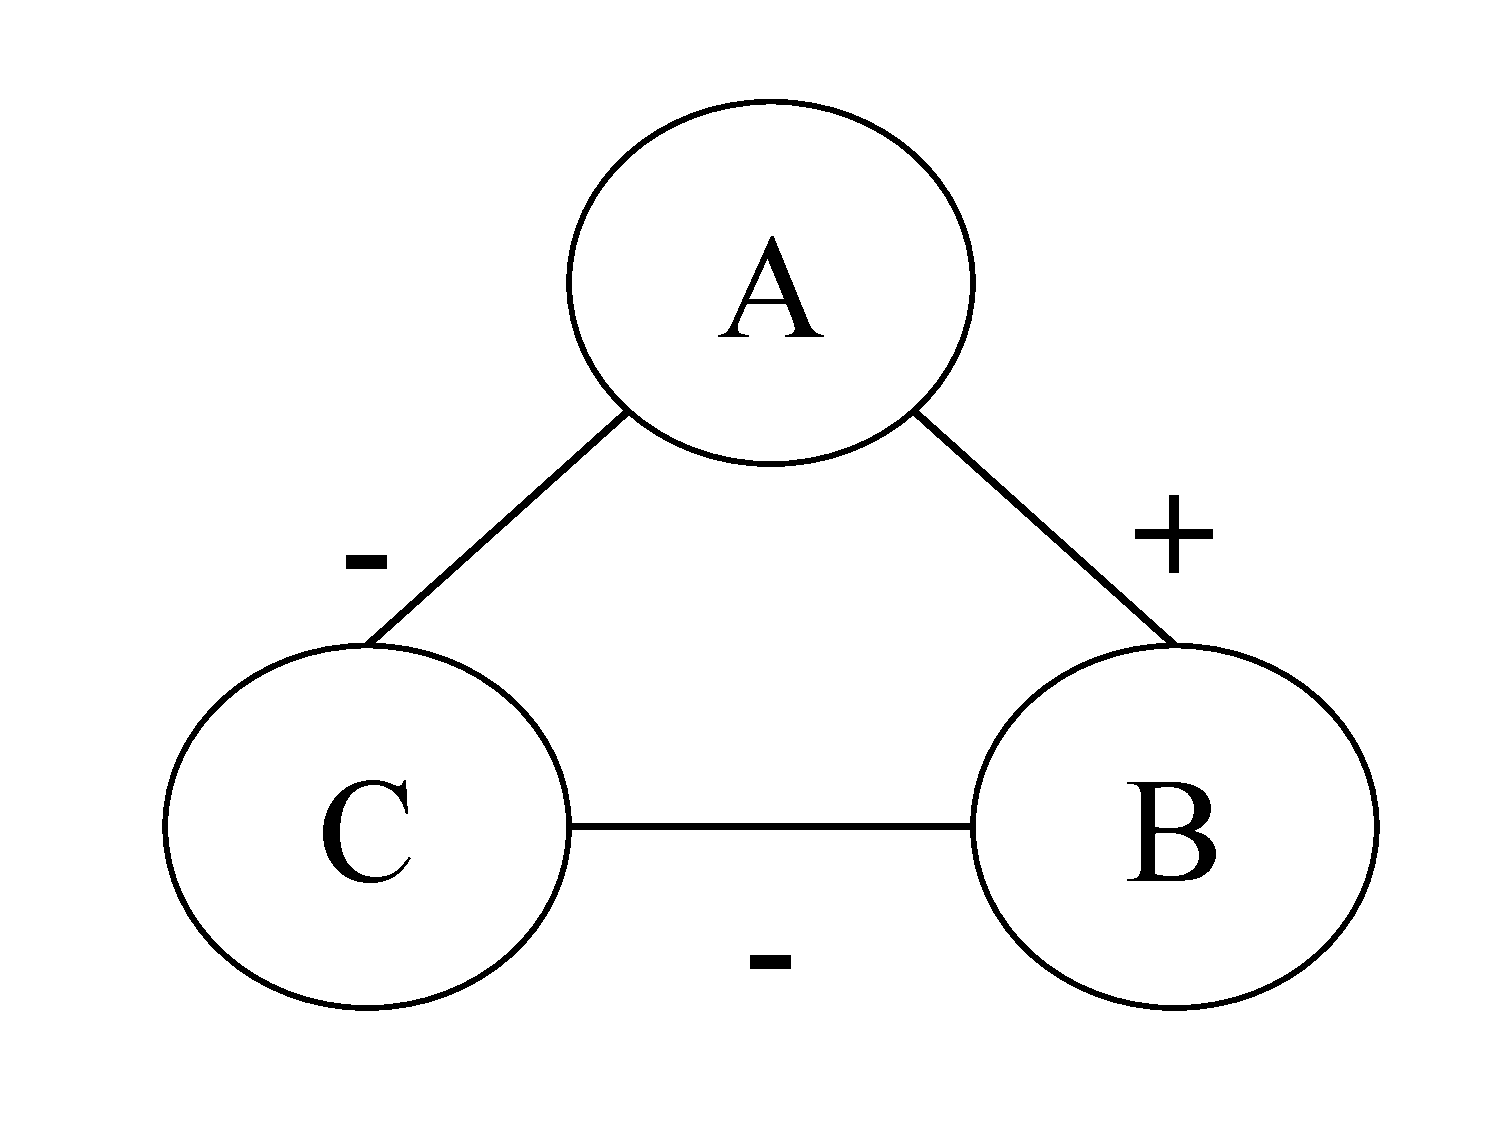
\includegraphics[scale=0.1]{balance_1P2N.pdf}
\label{fig:balance_1P2N}
}
\quad
\subfigure[$T_4$]{
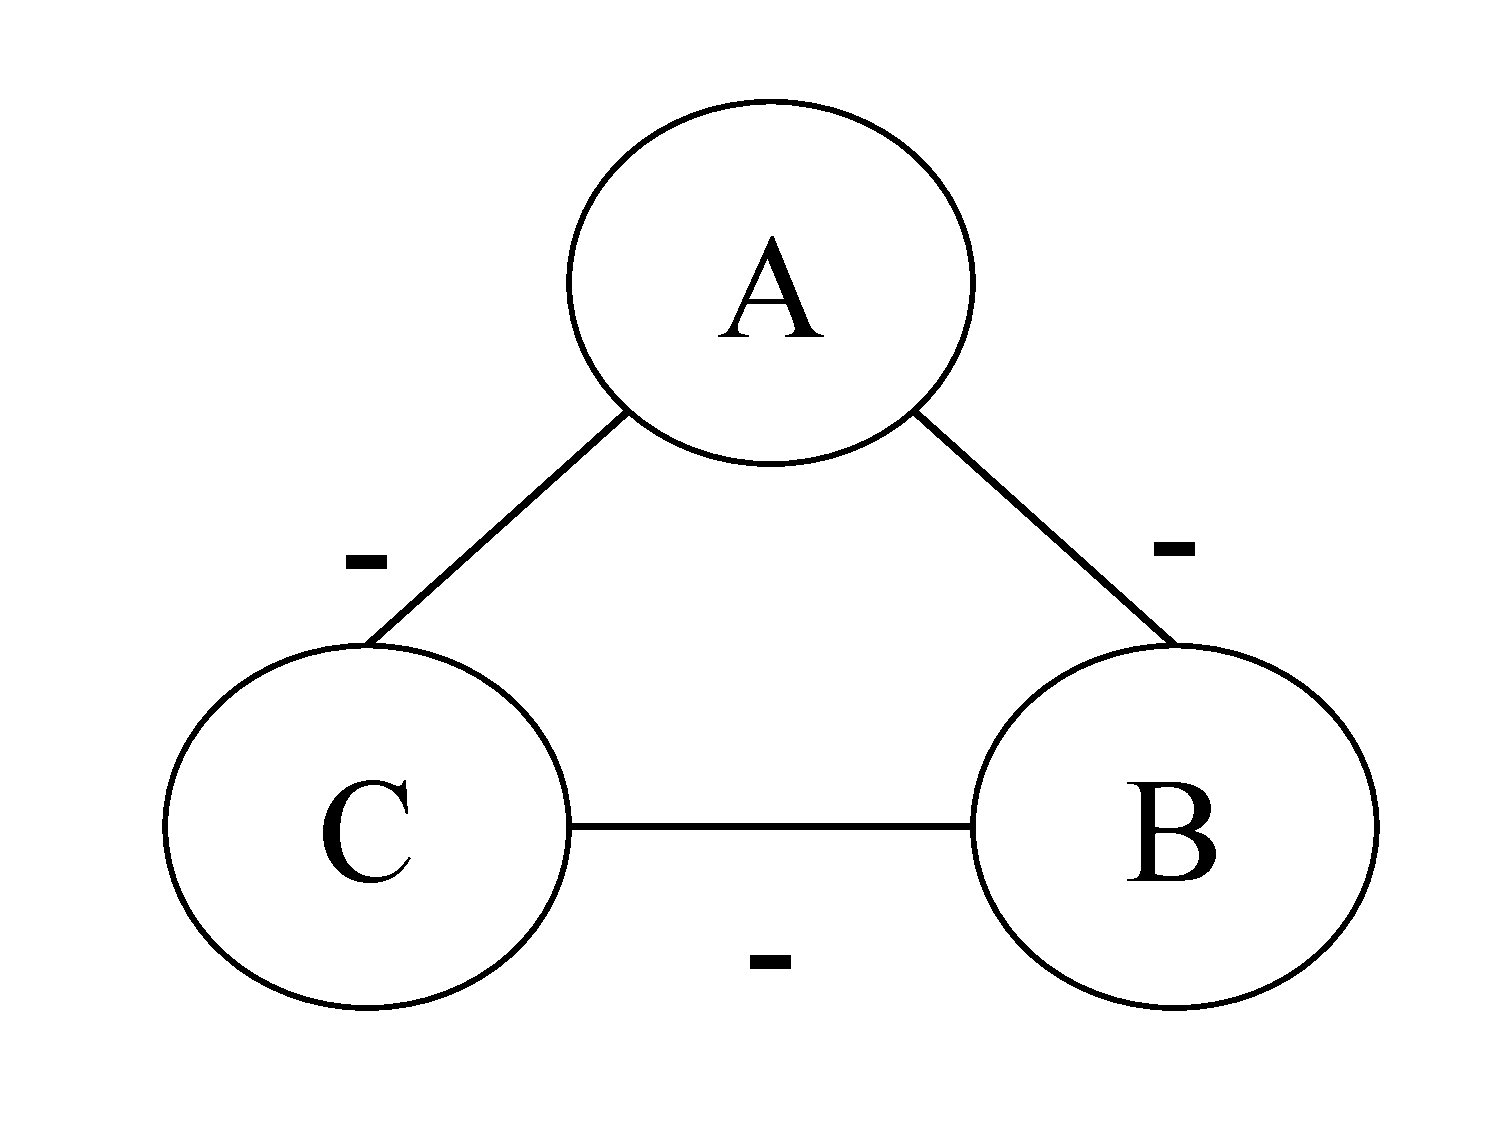
\includegraphics[scale=0.1]{balance_0P3N.pdf}
\label{fig:balance_1P2N}
}
\caption{Signed triads from balance theory. Triads $T_1$, and $T_3$ are \textit{balanced}, while triads $T_2$, and $T_4$ are \textit{unbalanced}}
\label{fig:balanceT}
\end{figure}

\begin{table}
\centering
% balance theory overall - AFINN
%('P', 'P', 'N') Study:  0.225961538462  Random:  0.451923076923
%('P', 'P', 'P') Study:  0.355769230769  Random:  0.125
%('N', 'N', 'N') Study:  0.1875  Random:  0.100961538462
%('P', 'N', 'N') Study:  0.230769230769  Random:  0.322115384615
\caption{Distribution of Balanced and Unbalanced Triads}
\begin{tabular}{| c | c | c |}
\hline
\textbf{Triad Type($T_i$)} & \textbf{$f_d(T_i)$} & \textbf{$f_r(T_i)$} \\
\hline
$T_1$ ($+++$) & 35.6\% & 12.5\%\\
\hline
$T_2$ ($++-$) & 22.6\% & 45.2\%\\
\hline
$T_3$ ($+--$) & 23.0\% & 32.2\%\\
\hline
$T_4$ ($---$)& 18.8\% & 10.1\%\\
\hline
\end{tabular}
\label{table:balanceTDist}
\end{table}

\subsection{Directed: Status Theory}